\documentclass[12pt,xcolor={usenames,dvipsnames}]{beamer}
\usetheme{Frankfurt}
%\usecolortheme{whale} % alterar esquema de cores
\useinnertheme{rectangles}

%%%%Código inserido para ter a barra com o nome da subseção abaixo da barra de navegação
\setbeamertemplate{headline}{
    % insere a barra de navegação
    \begin{beamercolorbox}[ht=2.125ex,dp=3.150ex]{section in head/foot}
        \insertnavigation{\paperwidth}
    \end{beamercolorbox}
    % insere a barra com o nome da subseção
    \setbeamercolor{bgcolor}{fg=white,bg=blue!20!black} 
    \begin{beamercolorbox}[ht=2.125ex,dp=1.125ex,leftskip=.3cm,rightskip=.3cm plus1fil]{bgcolor}
        \usebeamerfont{bgcolor}
        \insertsubsectionhead
    \end{beamercolorbox}%
}

%%%%Código inserido para ter a linha de rodapé junto do tema Frankfurt
\defbeamertemplate*{footline}{infolines theme}
{
    \leavevmode%
    \hbox{%
    \begin{beamercolorbox}[wd=.35\paperwidth,ht=2.25ex,dp=1ex,center]{author in head/foot}%
        \usebeamerfont{author in head/foot}

%se houver mais de 1 autor, o ideal é remover o nome dos autores da barra inferior
%\insertshortauthor~~

        \insertshortinstitute
    \end{beamercolorbox}%
    \begin{beamercolorbox}[wd=.3\paperwidth,ht=2.25ex,dp=1ex,center]{title in head/foot}%
        \usebeamerfont{title in head/foot}\insertshorttitle
    \end{beamercolorbox}%
    \begin{beamercolorbox}[wd=.35\paperwidth,ht=2.25ex,dp=1ex,right]{date in head/foot}%
        \usebeamerfont{date in head/foot}\insertshortdate{}\hspace*{2em}
        \insertframenumber{} / \inserttotalframenumber\hspace*{2ex}
    \end{beamercolorbox}
}%
%\vskip0pt%
}
%%%%%%%%%%%%%%%%%% 

\usepackage[utf8]{inputenc}
\usepackage[T1]{fontenc}
\usepackage[brazil]{babel}
\usepackage{tipa}
\usepackage{amssymb}
\usepackage{array}
\usepackage{bbold}
\usepackage{latexsym}
\usepackage{ae}
\usepackage{hyperref}
\usepackage{array}
\usepackage{booktabs}
\usepackage{graphicx}
\usepackage{dsfont}
\usepackage{textcomp}
\usepackage{cmll}
\usepackage[normalem]{ulem}
\usepackage{amsmath}
\usepackage{listings}
\usepackage{float}
\usepackage{upgreek}
\usepackage[portuguese]{algorithm2e}
\usepackage{tikz}
\usetikzlibrary{shapes,arrows,automata,positioning}
\usepackage{stmaryrd}
\usepackage{outlines}
\usepackage{mathrsfs} %fonte da sintaxe 
\newcommand{\CL}{$\mathcal{CL}$\xspace}
%\newcommand{\CLR}{$\mathcal{CL}$ Relativizada\xspace}
\newcommand{\RCL}{$\mathcal{RCL}$\xspace}
\newcommand{\RECALL}{$\mathcal{RECALL}$\xspace}
\newcommand\numberthis{\addtocounter{equation}{1}\tag{\theequation}}

\makeatletter
\newcommand{\miniscule}{\@setfontsize\miniscule{5}{6}}% \tiny: 5/6
\makeatother

\tikzstyle{tech} = [rectangle, draw, text width=7em, text centered]
\tikzstyle{obj} = [rectangle, draw, text width=5em, text centered, rounded corners,  fill=blue!60]  
\tikzstyle{final-logic} = [ellipse, draw, text width=9em, text centered, rounded corners, fill=blue!60]    
\tikzstyle{final-obj} = [rectangle, draw, text width=9em, text centered, rounded corners, fill=blue!60]    
\tikzstyle{line} = [draw, -latex]
\tikzstyle{logic} = [draw, ellipse, text centered]

\setcounter{secnumdepth}{3}
\setcounter{tocdepth}{3}

\lstset{
	backgroundcolor=\color{white},   % choose the background color; you must add \usepackage{color} or \usepackage{xcolor}
	basicstyle=\scriptsize,          % the size of the fonts that are used for the code
	breakatwhitespace=false,         % sets if automatic breaks should only happen at whitespace
	breaklines=true,                 % sets automatic line breaking
	captionpos=b,                    % sets the caption-position to bottom
	columns=flexible,
    deletekeywords={...},            % if you want to delete keywords from the given language
	escapeinside={\%*}{*)},          % if you want to add LaTeX within your code
	extendedchars=true,              % lets you use non-ASCII characters; for 8-bits encodings only, does not work with UTF-8
	frame=none,	                     % adds a frame around the code
	keepspaces=true,                 % keeps spaces in text, useful for keeping indentation of code
	language=Java,                   % the language of the code
	otherkeywords={*,...},           % if you want to add more keywords to the set
	numbers=left,                    % where to put the line-numbers; possible values are (none, left, right)
	numbersep=15pt,                  % how far the line-numbers are from the code
	numberstyle=\tiny,               % the style that is used for the line-numbers
	rulecolor=\color{black},         % if not set, the frame-color may be changed on line-breaks within not-black text
	showspaces=false,                % show spaces everywhere adding particular underscores; it overrides 'showstringspaces'
	showstringspaces=false,          % underline spaces within strings only
	showtabs=false,                  % show tabs within strings adding particular underscores
	stepnumber=1,                    % the step between two line-numbers. If it's 1, each line will be numbered
	tabsize=1	                     % sets default tabsize to 2 spaces
}

\lstdefinelanguage{rcl}{
    keywords=[1]{ O, P, F,CONFLICT,Trace,Stacktrace, AND, \^},
}

\lstdefinestyle{rcl}{
    basicstyle=\normalsize,
    numbers=left,
    numberstyle=\normalsize,
    numbersep=5pt,
    frame=lines,
    breaklines=true,
    prebreak=\raisebox{0ex}[0ex][0ex]{\ensuremath{\hookleftarrow}},
    showstringspaces=false,
    upquote=true,
    tabsize=1,
}

\usepackage[style=verbose,autocite=footnote]{biblatex}
\addbibresource{references.bib}


\title[\miniscule{Exame de Qualificação}]{Verificação formal para detecção de vulnerabilidades em contratos inteligentes}

\subtitle{}

\author{Gustavo Oliveira Dias\inst{1} \\ Prof. Dr. Adenilso da Silva Simão\inst{1}}

\institute[Universidade de São Paulo - USP]
{
    \inst{1}
Instituto de Ciências Matemáticas e de Computação - ICMC\\
}

\date[05 de julho de 2021]{05 de julho de 2021}

\subject{}

\AtBeginSubsection[]
{
    \addtocounter{framenumber}{-1}
    \begin{frame}{Sumário}
        \tableofcontents[currentsection,currentsubsection]
    \end{frame}
}

\begin{document}

\frame{\titlepage}

\begin{frame}{Sumário}
  \tableofcontents
  % possibilidade de adicionar opções [pausesections]
\end{frame}

%%%% Seções

\section{A tecnologia blockchain}
\subsection{Estrutura e funcionamento da blockchain}

\begin{frame}{Blockchain}
    \begin{block}{}
    \textbf{Blockchain} é o nome dado à tecnologia subjacente utilizada em diversas plataformas
    de gerenciamento descentralizado de posse de bens digitais baseada em \textbf{livro-razão distribuído}
    (do inglês, \textbf{\textit{Distributed Ledger Technology}} (DLT) )
    \end{block}
    Principais características:
    \begin{itemize}
        \item Armazenamento descentralizado e distribuído;
        \item Imutabilidade;
        \item Transparência;
        \item Dispensa da necessidade de confiança em uma terceira parte.
    \end{itemize}
\end{frame}

\begin{frame}{Blockchain Bitcoin}
    \begin{itemize}
        \item Primeiro caso de êxito: \textbf{Bitcoin};%\footnotemark[1];
            \item Criada em 2008 por Satoshi Nakamoto;
            \item Criptomoeda gerada e gerenciada de forma distribuída;
            \item Não possui entidades centralizadoras;
            \item Formada por uma rede de nós conectados auto-gerenciáveis;
            \item Nós trabalham para manter a integridade do sistema;
    \end{itemize}  
\end{frame}

\begin{frame}{Blockchain - Transações e blocos}
    \begin{itemize}
        \item Sempre que a posse de uma unidade ou fração de Bitcoin é transferida, uma \textbf{transação} é gerada;
        \item Quando uma nova transação ocorre, suas informações são transmitidas pela rede, tais como:
        \begin{itemize}
            \item Contas envolvidas;
            \item Quantia transferida;
            \item Assinatura digital;
            \item Horário da transação.
        \end{itemize}
        \item Os nós da rede, conhecidos como \textbf{mineradores}, coletam as transações e as armazenam em \textbf{blocos};
        \item Transações de um bloco são organizadas eu uma \textbf{árvore de Merkle}:
            \begin{itemize}
                \item Nós folhas: transações;
                \item Demais nós: Referências de \textit{hash}.
            \end{itemize}
    \end{itemize}
\end{frame}

\begin{frame}{Blockchain - Estrutura}
    \begin{figure}[!htb]
     \centering
     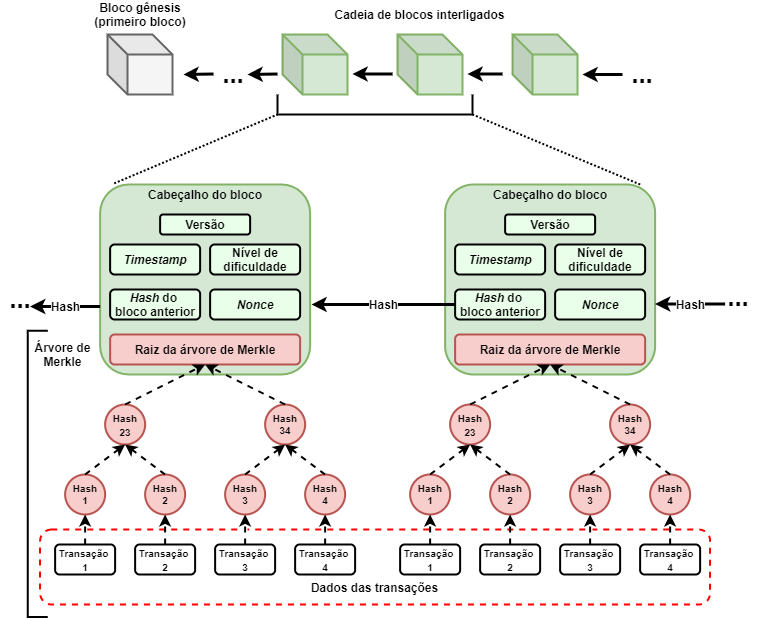
\includegraphics[scale=0.3]{figuras/blockchain/block_estrutura_cabeçalho.png}
    \end{figure}    
\end{frame}

\begin{frame}{Blockchain - Validação dos blocos}
    \begin{block}{Algoritmo de consenso}
    \begin{itemize}
        \item Regras a serem seguidas pelos nós para criação e validação dos blocos;
        \item Recompensa para os nós honestos;
        \item Garante que todos os nós da rede concordem com o histórico de transações que compõem os blocos da blockchain.
    \end{itemize}
    \end{block}    
\end{frame}

\begin{frame}{Blockchain - Algoritmos de consenso}
    \begin{exampleblock}{\textit{Proof-of-Work} (PoW)}
    \begin{itemize}
        \item Utilizado nas blockchains Bitcoin e Ethereum;
        \item Consiste na competição entre os mineradores para resolução do \textit{nonce} do bloco;
        \item O vencedor transmite o bloco pela rede para validação;
        \item Quanto maior o poder computacional do minerador, maior a chance de vencer;
        \item Resulta em um alto esforço computacional e gasto energético;
        \item O vencedor receber um valor da criptomoeda como recompensa (e.g., Bitcoin);
        \item \textbf{Desvantagem}: Esforço computacional elevado.
    \end{itemize}
    \end{exampleblock}
\end{frame}

% no final da explicação de blockchain, fazer um slide falando pq é difícil fraudar um bloco

\subsection{Blockchain Ethereum}

\begin{frame}{Ethereum}
    \begin{block}{}
    \begin{itemize}
        \item Apesar da blockchain ter sido criada para uma aplicação financeira (i.e., a Bitcoin), seus conceitos e protocolos podem ser estendidos para diversas áreas;
        \item É apenas um fim para um meio;
        \item Aplicações: Cuidados médicos, inteligência artificial, internet das coisas, governança descentralizada, entre outras.
    \end{itemize}
    \end{block}
    \begin{block}{}
    \begin{itemize}
        \item Em 2014 foi criada a blockchain \textbf{Ethereum};
        \item Introdução dos contratos inteligentes;
        \item Pioneira na expansão das aplicações da blockchain.
    \end{itemize}
    \end{block}
\end{frame}

\begin{frame}{Ethereum}
    \begin{itemize}
        \item Permite a geração, transferência e gerenciamento de sua criptomoeda, o \textbf{Ether};
        \item Seu funcionamento é baseado na implantação dos \textbf{contratos inteligentes} (CI):
        \begin{itemize}
            \item Programas de computador;
            \item Executam automatica e obrigatoriamente aquilo que foi programado;
            \item Estabelecem um acordo entre os envolvidos;
            \item Geração de transações.
        \end{itemize}
	    \item Opera de forma semelhante à Bitcoin na garantia da \textbf{imutabilidade}.
    \end{itemize}
\end{frame} 

%\begin{frame}{Ethereum}
%    \begin{itemize}
%        \item Aplicações Descentralizadas (do inglês, \textit{Descentralized Applications} (DApps)):
%        \begin{itemize}
%            \item Mais de 3 mil utilizam a Ethereum~\footnote{\url{<https://www.stateofthedapps.com/>}}.
%        \end{itemize}
%    \end{itemize}
%\end{frame}

\begin{frame}{Ethereum - Propriedades}
    As aplicações que executam sobre a Ethereum dispõem de uma série de propriedades:
    \begin{itemize}
        \item Descentralização;
        \item Imutabilidade;
        \item Persistência de dados;
        \item Execução autônoma;
        \item Acurácia.
    \end{itemize}
\end{frame}

\begin{frame}{Ethereum - Aplicações}
    \begin{itemize}
        \item Sistema de \textbf{tokens}:
        \begin{itemize}
            \item Tokenização;
            \item Padrão ERC-20.
        \end{itemize}
        \item Organização Autônoma Descentralizada:
        \begin{itemize}
            \item Regras operacionais e de gerenciamento são programadas em um CI;
            \item Abolição de modelos baseados em hierarquia;
            \item Redução de custos;
            \item Primeira OAD: \textit{The DAO}.
        \end{itemize}
        \item Cuidados médicos e serviços de saúde:
        \begin{itemize}
            \item Integração de dados de prontuários.
        \end{itemize}
    \end{itemize}
\end{frame}

%\begin{frame}{Ethereum - Arquitetura em camadas}
%    \begin{figure}[!htb]
%     \centering
%     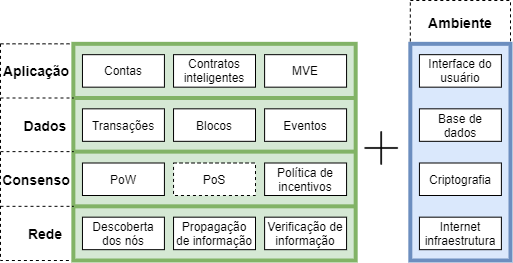
\includegraphics[scale=0.5]{figuras/blockchain/ethereum_arquitetura.png}
%    \end{figure}    
%\end{frame}
\section{Contratos inteligentes}
\subsection{Fundamentos}

\begin{frame}{Contratos inteligentes}
    \begin{itemize}
        \item 1997: Primeira proposta;
        \item 2014: Primeira aplicação - blockchain Ethereum;
        \item Outras plataformas que implementam CIs: Hyperledger Fabric, Corda e Stellar.
    \end{itemize}
    \begin{block}{Desenvolvimento de um CI}
    Cláusulas contratuais estabelecidas em comum acordo entre as partes envolvidas são expressas por meio de programas de computador executáveis.
    \end{block}
    \begin{itemize}
        \item Solidity: linguagem desenvolvida para CIs na Ethereum;
        \item CIs são sempre compilados para \textit{bytecode};
        \item O \textit{bytecode} é executado na MVE.
    \end{itemize}
\end{frame}

\begin{frame}{Contratos inteligentes}
    \begin{figure}[!htb]
     \centering
     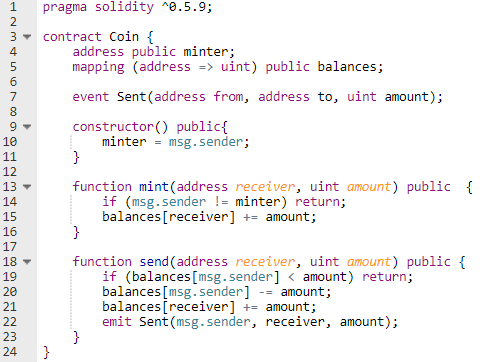
\includegraphics[scale=0.6]{figuras/contratos-inteligentes/exemplo_codigo_solidity.png}
    \end{figure}
\end{frame}

\begin{frame}{Contratos inteligentes}
    \begin{block}{}
    A utilização dos CIs possui um ciclo de vida de quatro fases: \textbf{criação}; \textbf{implantação}; \textbf{execução}; e \textbf{conclusão}.
    \end{block}
    \begin{figure}[!htb]
        \centering
        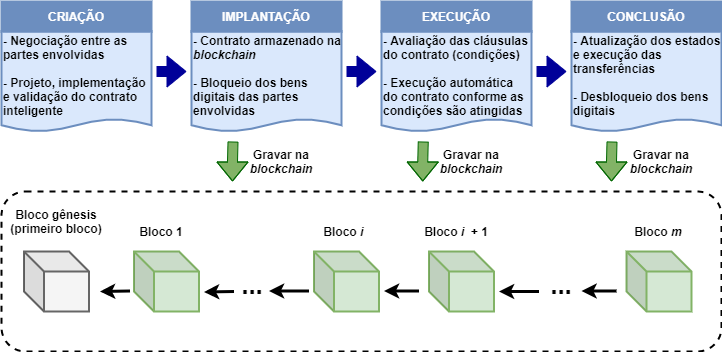
\includegraphics[scale=0.4]{figuras/contratos-inteligentes/contrato_ciclo_de_vida.png}
    \end{figure}    
\end{frame}

\subsection{Vulnerabilidades e ataques}

\begin{frame}{Contratos inteligentes}
    \begin{block}{}
    Devido à \textbf{imutabilidade} da blockchain, um contrato implementado não pode mais ser alterado.
    \end{block}
    \begin{block}{}
    Esta propriedade agrega \textbf{integridade} à tecnologia blockchain, mas também ressalta a importância da implementação de contratos livres de erros e de acordo com boas práticas.
    \end{block}
    \begin{block}{}
	Aplicações desenvolvidas por meio de CIs costumam envolver transferências e gerenciamento de grandes quantias em Ether.
	\end{block}
    \begin{alertblock}{}
    \textbf{Vulnerabilidades} deixadas nos códigos dos CIs podem torná-los alvos de \textbf{ataques}.
    \end{alertblock}
\end{frame}

\begin{frame}{Contratos inteligentes - Vulnerabilidades e ataques}
    \begin{itemize}
        \item Primeiro ataque: \textit{The DAO Attack} (2016);
        \item Vulnerabilidade explorada: \textbf{Reentrância};
        \item Um usuário malicioso transferiu \textbf{3,6 milhões} em Ether para sua conta;
        \item Equivalente a \textbf{50 milhões} de dólares.
    \end{itemize}
    \begin{block}{}
    Este caso teve grande repercussão e motivou estudos e estratégias para \textbf{detecção} e \textbf{prevenção} de \textbf{vulnerabilidades} em CIs. 
    \end{block}
\end{frame}

\begin{frame}{Contratos inteligentes - Vulnerabilidades e ataques}
    \begin{block}{}
    Parte dos erros e vulnerabilidades explorados em ataques contra os CIs são ocasionados pelo desalinhamento que há entre a semântica da linguagem Solidity e a intuição dos desenvolvedores.
    \end{block}
    \begin{block}{}
    Solidity possui elementos similares ao de outras linguagens, mas que não são implementados da mesma forma.
    \end{block}
    \begin{alertblock}{}
    Há registro de uma série de vulnerabilidades que resultaram na exploração de CIs e enormes perdas financeiras.
    \end{alertblock}
\end{frame}

\begin{frame}{Contratos inteligentes - Vulnerabilidades e ataques}
    Vulnerabilidades alvos desta pesquisa:
    \begin{itemize}
        \item Reentrância;
        \item \textit{Delegatecall injection};
        \item Contrato suicida.
    \end{itemize}
\end{frame}

\begin{frame}{Vulnerabilidade - Reentrância}
    \begin{itemize}
        \item Explorada no \textit{The DAO Attack};
        \item Pode ocorrer quando um contrato pode ser invocado recursivamente sucessivas vezes;
        \item Ocorre por meio de uma função \textit{callback}.
    \end{itemize}
    \begin{figure}[!htb]
        \centering
        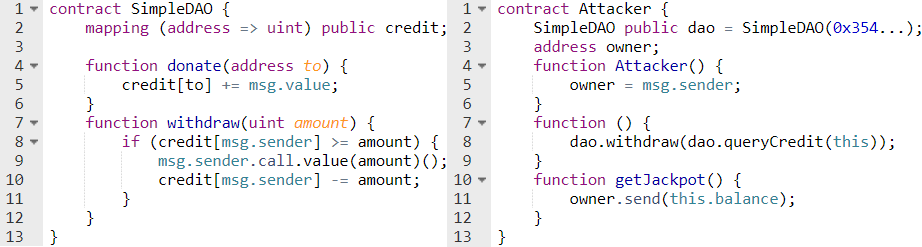
\includegraphics[scale=0.45]{figuras/contratos-inteligentes/reentrancia-exemplo.png}
    \end{figure}
\end{frame}

\begin{frame}{Exploração da reentrância}
    \begin{itemize}
        \item 1º Passo: Publicação do contrato.
    \end{itemize}
    \begin{figure}[!htb]
     \centering
     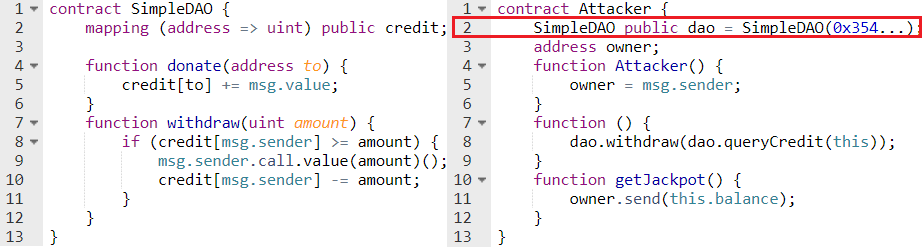
\includegraphics[scale=0.45]{figuras/contratos-inteligentes/reentrancia-passo-1.png}
    \end{figure}    
\end{frame}

\begin{frame}{Exploração da reentrância}
    \begin{itemize}
        \item 2º Passo: Doação para o contrato utilizando sua conta.
    \end{itemize}
    \begin{figure}[!htb]
     \centering
     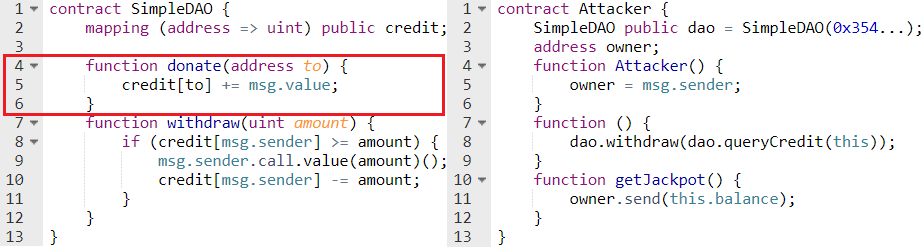
\includegraphics[scale=0.45]{figuras/contratos-inteligentes/reentrancia-passo-2.png}
    \end{figure}     
\end{frame}

\begin{frame}{Exploração da reentrância}
    \begin{itemize}
        \item 3º Passo: Invocação da função \textit{fallback}, que invoca a função \texttt{withdraw};
        \item Ether é transferido para o \texttt{Attacker}.
    \end{itemize}
    \begin{figure}[!htb]
     \centering
     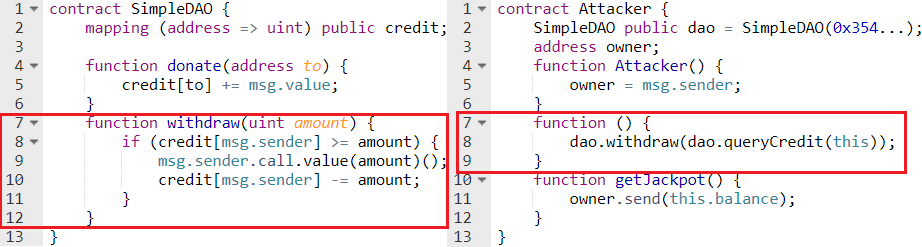
\includegraphics[scale=0.45]{figuras/contratos-inteligentes/reentrancia-passo-3.png}
    \end{figure}     
\end{frame}

\begin{frame}{Exploração da reentrância}
    \begin{itemize}
        \item 4º Passo: Chamadas sucessivas à função \texttt{withdraw}.
        \item Da forma como é usada, a função \texttt{call}, que é uma função \textit{callback}, permite nova invocação da função \texttt{withdraw} antes da execução do comando \texttt{credit[msg.sender] -= amount};
        \item Verificação da linha 8 tem êxito novamente.
    \end{itemize}
    \begin{figure}[!htb]
     \centering
     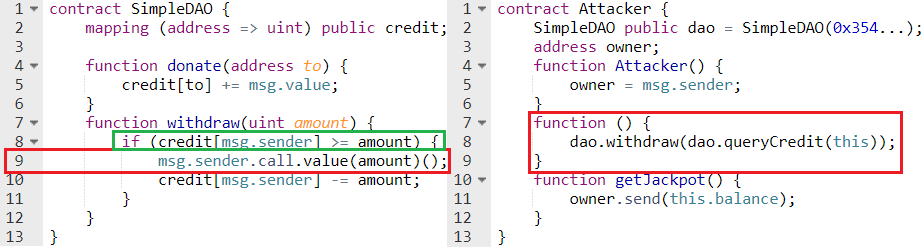
\includegraphics[scale=0.45]{figuras/contratos-inteligentes/reentrancia-passo-4.png}
    \end{figure}     
\end{frame}

\begin{frame}{Exploração da reentrância}
    \begin{itemize}
        \item As transferências são realizadas sucessivamente até ocorrer um dos seguintes eventos:
        \begin{itemize}
            \item Todo \textit{gas} é utilizado;
            \item Pilha de chamadas da MVE é totalmente preenchida;
            \item Saldo do \texttt{SimpleDAO} é zerado.
        \end{itemize}
        \item Como evitar:
        \begin{itemize}
            \item Atualizar as variáveis de estado antes da invocação de outro contrato;
            \item Trava \textit{mutex};
            \item Utilizar o método \texttt{transfer}.
        \end{itemize}
    \end{itemize}
    \begin{block}{}
    Os danos causados pelo \textit{The DAO Attack} foram revertidos por meio de um \textit{hard fork}, que causou uma divisão dos mineradores da Ethereum.
    \end{block}
\end{frame}

\begin{frame}{Vulnerabilidade - \textit{Delegatecall injection}}
    \begin{itemize}
        \item Explorada no ataque contra a \textit{Parity Multsignature Wallet};
        \item Em 2017, 31 milhões de dólares foram subtraídos em um ataque;
        \item \texttt{delegatecall}: Usado para inserir o \textit{bytecode} de um contrato no \textit{bytecode} de outro contrato;
        \item O contrato que é chamado pode alterar as variáveis de estado do contrato que o invocou;
        \item O invasor atribuiu para si a posse do contrato e realizou a transferência para sua conta.
    \end{itemize}
\end{frame}

%\begin{frame}{Exploração da \textit{delegatecall injection}}
%    \begin{figure}[!htb]
%     \centering
%     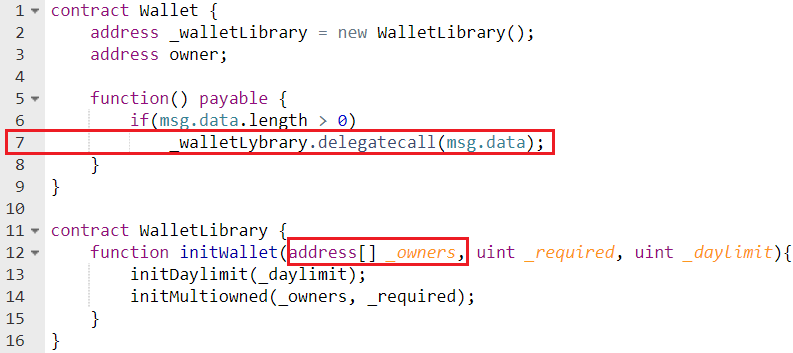
\includegraphics[scale=0.5]{figuras/contratos-inteligentes/delegatecall-passo1.png}
%    \end{figure}    
%\end{frame}

%\begin{frame}{Exploração da \textit{delegatecall injection}}
%    \begin{itemize}
%        \item Envio de uma transação com o campo \texttt{msg.data} contendo \texttt{initWallet} como a função a ser chamada;
%        \item Os endereços de posse do contrato (\texttt{\_owners}) foram substituídos pelo endereço do atacante;
%        \item Foi realizada a transferência de 31 milhões de dólares em Ether.
%        \item Como evitar: 
%        \begin{itemize}
%            \item Declarar contrato a ser compartilhado (\texttt{WalletLibrary}) como uma biblioteca (\texttt{library}).
%        \end{itemize}
%    \end{itemize}
%\end{frame}

\begin{frame}{Vulnerabilidade - Contrato suicida}
    \begin{itemize}
        \item Um contrato pode ser ``morto'' pelo dono do contrato ou outra parte confiável;
        \item Métodos: \texttt{suicide} ou \texttt{selfdestruct};
        \item O \textit{bytecode} e o armazenamento do contrato é deletado;
        \begin{block}{}
        A vulnerabilidade \textbf{contrato suicida}, acontece quando uma \textbf{autenticação inadequada} permite que algum invasor tome posse do contrato e execute a função para matar o contrato.
        \end{block}
        \item Foi explorada em um segundo ataque contra a \textit{Parity Wallet};
        \item \textbf{280 milhões} de dólares em Ether foram permanentemente \textbf{bloqueados}.
    \end{itemize}
\end{frame}

%\begin{frame}{Exploração da vulnerabilidade contrato suicida}
%    \begin{itemize}
%        \item Como resposta ao primeiro ataque, foi adicionado o modificador \texttt{only\_uninitialized};
%        \item Porém, o contrato \texttt{WalletLibrary} foi deixado como não inicializado;
%        \item O invasor passou pelo modificador, se declarou dono do contrato, e invicou o método suicide.
%    \end{itemize}
%    \begin{figure}[!htb]
%     \centering
%     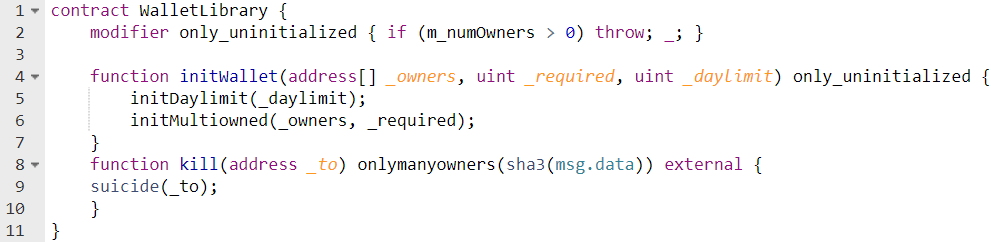
\includegraphics[scale=0.4]{figuras/contratos-inteligentes/parity-corrigido.png}
%    \end{figure}    
%\end{frame}

\begin{frame}{Ethereum - Vulnerabilidades}
    \begin{block}{}
    Além da reentrância, \textit{delegatecall injection} e contrato suicida, existem diversas outras vulnerabilidades encontradas na literatura, e que devem ser evitadas.
    \end{block}
    \begin{block}{}
    Desde o \textit{The DAO Attack}, muitos esforços foram realizados para desenvolvimento de métodos, ferramentas e frameworks para \textbf{verificação de CIs} e \textbf{detecção de vulnerabilidades}.
    \end{block}
	\begin{exampleblock}{Questão de pesquisa}
	Como detectar as vulnerabilidades de \textbf{reentrância}, \textbf{\textit{delegatecall injection}} e \textbf{contrato suicida}, em CIs escritos na linguagem \textbf{Solidity} na fase de \textbf{pré-implantação}?	
	\end{exampleblock}
\end{frame}


\section{Verificação e validação}
\subsection{Métodos de verificação}

\begin{frame}{Vulnerabilidades em CIs}
    \begin{block}{}
    Grande parte das vulnerabilidades encontradas em CIs escritos em Solidity poderiam ter sido evitadas com a ajuda de \textbf{análise formal} e \textbf{verificação} desses contratos antes de serem implantados na blockchain.
    \end{block}
    \begin{itemize}
        \item Linguagens como Solidity não foram desenvolvidas para serem verificadas formalmente;
        \item Solidity não é uma linguagem perfeita;
        \item Questões relacionadas com a execução dos CIs na Ethereum muitas vezes não são compreendidas pelos desenvolvedores.
    \end{itemize}
\end{frame}

\begin{frame}{Vulnerabilidades em CIs - Como evitar?}
    \textbf{Serviços de auditoria:}
    \begin{itemize}
        \item Organizações: OpenZeppeling, Solidified e SmartDec;
        \item Podem ser muito custosos para pequenas organizações e desenvolvedores autônomos.
    \end{itemize}
    \begin{exampleblock}{\textbf{Solução}}
    \textbf{Frameworks e ferramentas de verificação de CIs}
    \end{exampleblock}
\end{frame}

\begin{frame}{Verificação de CIs - Frameworks e ferramentas}
    Dois tipos de verificação:
    \begin{itemize}
        \item Proativa:
        \begin{itemize}
            \item Aplicada antes da implantação.
        \end{itemize}
        \item Reativa:
        \begin{itemize}
            \item Monitoramento do contrato durante a execução;
            \item Verificação em \textbf{tempo de execução}.
        \end{itemize}
    \end{itemize}
\end{frame}

\begin{frame}{Verificação de CIs - Frameworks e ferramentas}
	Métodos de verificação:
	\begin{itemize}
		\item Análise de código:
		\begin{itemize}
			\item Pode ser \textbf{estática}, \textbf{dinâmica} ou \textbf{híbrida};
			\item \textbf{Execução simbólica}.
		\end{itemize}
		\item Métodos formais:
		\begin{itemize}
			\item \textit{Model checking};
			\item Demonstração de teoremas;
			\item Verificação dedutiva.
		\end{itemize}		
	\end{itemize}
\end{frame}

\begin{frame}{Análise de código}
	\begin{itemize}
		\item Estratégia geralmente automatizada;
		\item Detecção de erros;
		\item Identificação de vulnerabilidades;
		\item Aspectos analisados:
		\begin{itemize}
			\item Fluxo de controle;
			\item Fluxo de dados;
			\item Interface;
			\item Fluxo de informações;
			\item Caminhos de execução.
		\end{itemize}
		\item Verificação pode ser \textbf{estática}, \textbf{dinâmica} ou \textbf{híbrida};
		\item Normalmente é utilizada alguma representação intermediária estruturada:
		\begin{itemize}
			\item Grafo de fluxo de controle;
			\item Árvore sintática em XML.
		\end{itemize}
		\item \textbf{Execução simbólica}.
	\end{itemize}
\end{frame}

\begin{frame}{\textit{Model checking}}
	\begin{itemize}
		\item Verificação de sistemas de transição de estados;
		\item Três etapas:
		\begin{itemize}
			\item Modelagem;
			\item Especificação: especificação formal dos requisitos;
			\begin{itemize}
				\item Propriedades: Lógicas temporais.
			\end{itemize}
			\item Verificação.
		\end{itemize}
	\end{itemize}
	\begin{figure}[!htb]
		\centering
		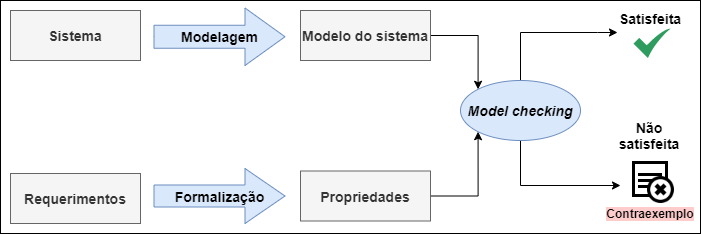
\includegraphics[scale=0.4]{figuras/verificacao/model-checking.png}
	\end{figure}    
\end{frame}

\begin{frame}{Verificação de CIs - Frameworks e ferramentas}
	Métodos de verificação:
	\begin{itemize}		
		\item \textit{Fuzzing}:
		\begin{itemize}
			\item Geração de mutações.
		\end{itemize}
		\item Técnicas de Inteligência Artificial (IA):
		\begin{itemize}
			\item \textit{Machine learning} e \textit{deep learning}.
		\end{itemize}
		\item Em tempo de execução:
		\begin{itemize}
			\item Instrumentalização de código.
		\end{itemize}
	\end{itemize}
\end{frame}


\section{Metodologia}
\subsection{Técnicas de pesquisa}

\begin{frame}{Objetivo da pesquisa}
	\begin{block}{Objetivo geral}
		Propor uma estratégia para verificação formal para aprimoramento de segurança aplicada na fase de pré-implantação de CIs escritos em \textbf{Solidity} para detecção das vulnerabilidades de \textbf{reentrância}, \textbf{\textit{delegatecall injection}} e \textbf{contrato suicida}, por meio da técnica de \textbf{\textit{model checking}}.
	\end{block}
	%	Objetivos específicos:
	%	\begin{itemize}
	%		\item Determinar o formalismo adequado para modelagem dos contratos e para representação das vulnerabilidades;
	%		\item Implementar o método de verificação;
	%		\item Definir as estratégias para validação da proposta.
	%	\end{itemize}
\end{frame}

\begin{frame}{Metodologia e técnicas de pesquisa}
    \begin{block}{Objetivo do Mapeamento Sistemático (MS) realizado}
    Identificar e classificar o conteúdo relacionado à \textbf{verificação para correção} ou \textbf{detecção de vulnerabilidades} para aprimoramento da segurança dos CIs.
    \end{block}
    Fundamentado no MS:
    \begin{itemize}
        \item Seleção do método de verificação e detecção de vulnerabilidades;
        \item Seleção das vulnerabilidades abordadas;
        \item Definição da estratégia para validação da proposta. 
    \end{itemize}
\end{frame}

\subsection{Mapeamento Sistemático}
\begin{frame}{Mapeamento Sistemático}
    Três fases:
    \begin{itemize}
        \item Planejamento;
        \item Condução;
        \item Publicação dos resultados.
    \end{itemize}
    \begin{figure}[!htb]
		\centering
		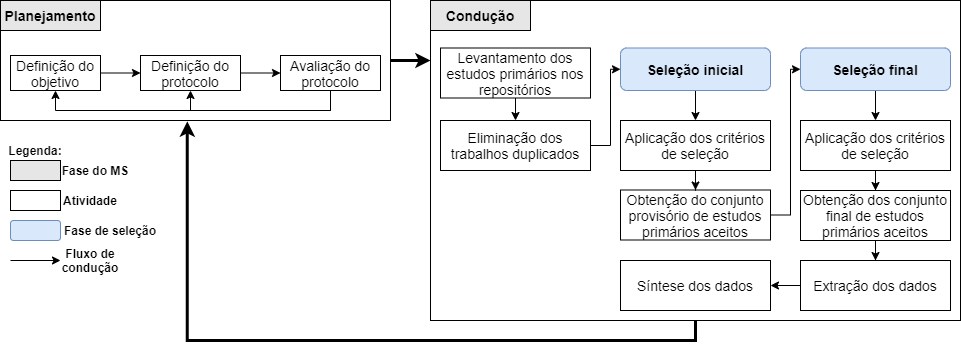
\includegraphics[scale=0.3]{figuras/metodologia/ms_fluxo.png}
	\end{figure}
\end{frame}

\begin{frame}{Protocolo do MS}
\textbf{Questões de pesquisa}:
    \begin{itemize}
        \item \textbf{QP 1.} Quais \textbf{abordagens} têm sido propostas?
        \item \textbf{QP 2.} \textbf{Quando} e \textbf{onde} os estudos têm sido publicados?
        \item \textbf{QP 3.} Quais \textbf{problemas} ou \textbf{vulnerabilidades} relacionados aos CIs têm sido abordados?
        \item \textbf{QP 4.} Quais \textbf{estratégias de validação} foram utilizadas?
        \item \textbf{QP 5.} Quais são as \textbf{limitações} presentes nas abordagens?
    \end{itemize}    
\end{frame}

\begin{frame}{Protocolo do MS}
\textbf{String de busca}:
    \begin{center}
    (\textit{``smart contract'' OR ``ethereum bytecode''}) \textit{AND} (\textit{verification OR validation OR monitor* OR analysis OR formalization OR ``formal methods'' OR ``security vulnerabilities'' OR ``security bugs'' OR ``vulnerability detection'' OR ``bug detection'' OR optimiz*})
    \end{center}
\textbf{Motores de busca e bases bibliográficas}:
    \begin{itemize}
        \item \textit{Engineering Village};
        \item \textit{Scopus};
        \item \textit{Web of Science};
        \item \textit{IEEE Xplore};
        \item \textit{ACM Digital Library}.
    \end{itemize}
\end{frame}

\begin{frame}{Planejamento e condução}
    \begin{itemize}
        \item Total de estudos selecionados: 2091
        \item Total de estudos aceitos: \textbf{104}
    \end{itemize}
\end{frame}

\begin{frame}{Discussão - \textit{Model checking}}
    \begin{itemize}
        \item \textbf{Está entre as abordagens mais utilizadas nos últimos anos};
        \item Há poucos estudos com validação experimental;
        \item Reentrância foi a vulnerabilidade mais abordada;
        \item Violação de propriedades:
        \begin{itemize}
        	\item Amplamente abordada;
        	\item Principalmente \textit{model checking}.
        \end{itemize}
    	\item Está entre as que apresentam melhor precisão e acurácia.
    \end{itemize}
\end{frame}

\begin{frame}{Discussão - \textit{Model checking}}
    \begin{figure}[!htb]
		\centering
		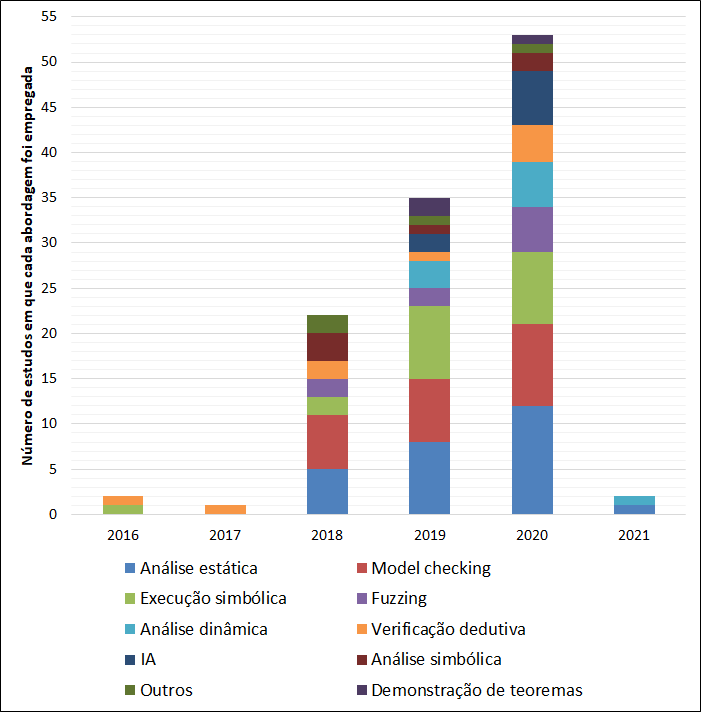
\includegraphics[scale=0.35]{figuras/metodologia/rq2-distribuicao-abordagens.png}
	\end{figure}
\end{frame}

\begin{frame}{Discussão - \textit{Model checking}}
    \begin{figure}[!htb]
		\centering
		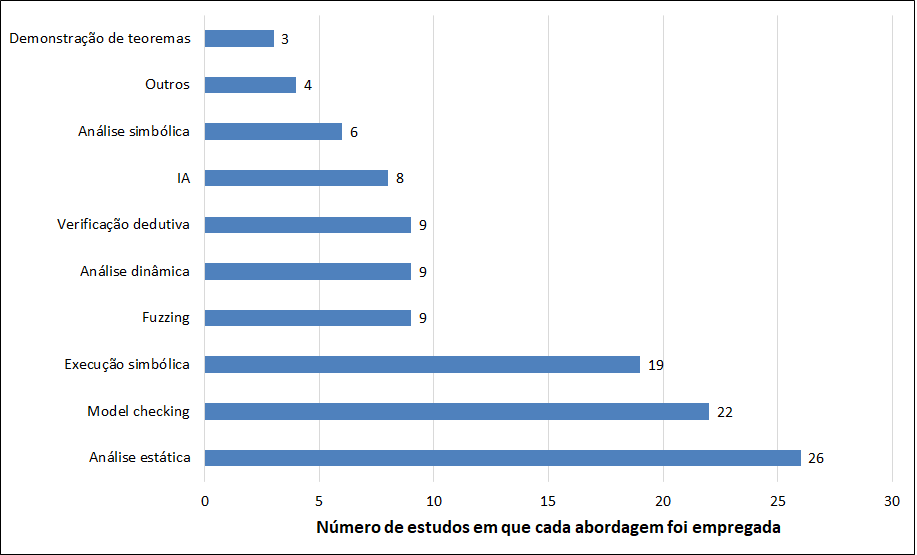
\includegraphics[scale=0.4]{figuras/metodologia/rq1-abordagens.png}
	\end{figure}
\end{frame}

\begin{frame}{Discussão - \textit{Model checking}}
	\begin{itemize}
		\item Está entre as abordagens mais utilizadas nos últimos anos;
		\item \textbf{Há poucos estudos com validação experimental};
		\item Reentrância foi a vulnerabilidade mais abordada;
		\item Violação de propriedades:
		\begin{itemize}
			\item Amplamente abordada;
			\item Principalmente \textit{model checking}.
		\end{itemize}
		\item Está entre as que apresentam melhor precisão e acurácia.
	\end{itemize}
\end{frame}

\begin{frame}{Discussão - \textit{Model checking}}
    \begin{figure}[!htb]
		\centering
		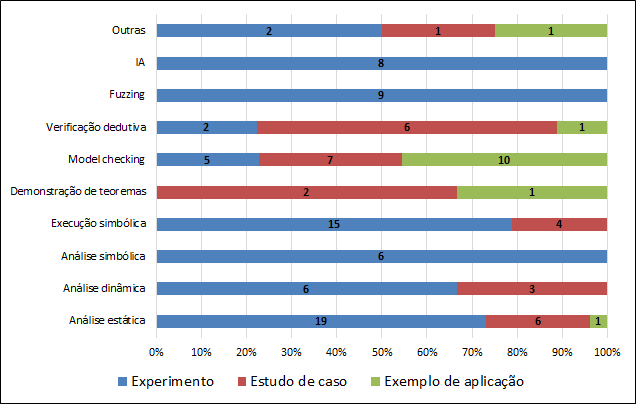
\includegraphics[scale=0.5]{figuras/metodologia/rq4-validacao-propostas.png}
	\end{figure} 
\end{frame}

\begin{frame}{Discussão - \textit{Model checking}}
	\begin{itemize}
		\item Está entre as abordagens mais utilizadas nos últimos anos;
		\item Há poucos estudos com validação experimental;
		\item \textbf{Reentrância foi a vulnerabilidade mais abordada};
		\item \textbf{Violação de propriedades}:
		\begin{itemize}
			\item Amplamente abordada;
			\item Principalmente \textit{model checking}.
		\end{itemize}
		\item Está entre as que apresentam melhor precisão e acurácia.
	\end{itemize}
\end{frame}

\begin{frame}{Discussão - \textit{Model checking}}
    \begin{figure}[!htb]
		\centering
		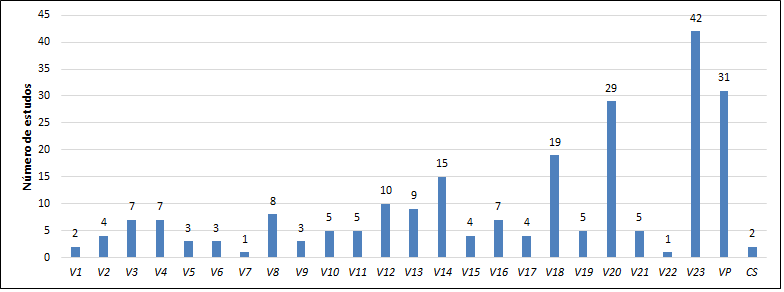
\includegraphics[scale=0.55]{figuras/metodologia/rq3-vulnerabilidades.png}
	\end{figure}
\end{frame}

\begin{frame}{Discussão - \textit{Model checking}}
	\begin{table}[!ht]
\centering
\fontsize{8pt}{8pt}\selectfont
\caption{Vulnerabilidades e problemas alvos de verificação em CIs}
\label{tab:rq3-vulnerabilidades}
\begin{tabular}{@{}llll@{}}
\toprule
\textbf{Sigla} & \textbf{Vulnerabilidade / Problema} & \textbf{Sigla} & \textbf{Vulnerabilidade / Problema} \\ \midrule
$V_{1}$  & Ataque de profundidade da pilha de chamadas & $V_{14}$ & Dependência de \textit{timestamp}       \\
$V_{2}$  & Ataque DoS com operações ilimitadas         & $V_{15}$ & Desordem de exceções           \\
$V_{3}$  & Autenticação com \textit{tx.origin}                  & $V_{16}$ & Divisão por zero               \\
$V_{4}$  & Bloqueio de Ether                           & $V_{17}$ & Endereço curto                 \\
$V_{5}$  & Consumo de \textit{gas} ineficiente                  & $V_{18}$ & Exceções não tratadas          \\
$V_{6}$  & Contrato guloso                             & $V_{19}$ & Chamada externa não verificada \\
$V_{7}$  & Contrato pródigo                            & $V_{20}$ & \textit{Integer overflow} e \textit{underflow}   \\
$V_{8}$  & Contrato suicida                            & $V_{21}$ & Gasto de \textit{gas} descontrolado     \\
$V_{9}$  & Contrato \textit{honeypot}                           & $V_{22}$ & Problemas de concorrência      \\
$V_{10}$ & Controle de acesso vulnerável               & $V_{23}$ & Reentrância                    \\
$V_{11}$ & \textit{Delegatecall injection}             & $VP$  & Violação de propriedades       \\
$V_{12}$ & Dependência de informação do bloco          & $CSS$ & Correção sintática e semântica \\
$V_{13}$ & Dependência de ordem da transação           &       &                                \\ \bottomrule
\end{tabular}
\end{table} 
\end{frame}   

\begin{frame}{Discussão - \textit{Model checking}}
	\begin{itemize}
		\item Está entre as abordagens mais utilizadas nos últimos anos;
		\item Há poucos estudos com validação experimental;
		\item Reentrância foi a vulnerabilidade mais abordada;
		\item Violação de propriedades:
		\begin{itemize}
			\item Amplamente abordada;
			\item Principalmente \textit{model checking}.
		\end{itemize}
		\item \textbf{Está entre as que apresentam melhor precisão e acurácia.}
	\end{itemize}
\end{frame}


%abrangência
%nível de automação
%conhecimento prévio
%acurácia - FP ou FN

- Model checking

- Entrada: código solidity e bytecode

 - Vulnerabilidades:
    Reentrância
    Delegatecall
    Contrato suicida
    Violação de propriedades funcionais
    
 
\frame{\titlepage}
 
\end{document}
